\chapter{Open Systems Interconnection (OSI)}

The Open Systems Interconnection (OSI) model is a conceptual framework developed by the International Standards Organization (ISO) in 1978. It describes the seven layers involved in networking to standardize communication across diverse systems.

\section{Layers of OSI}

\subsection{Physical Layer}
The Physical Layer is the lowest layer of the OSI model. It is responsible for the actual physical connection between devices. This layer defines the hardware means of sending and receiving data on a carrier, including the layout of pins, voltages, cable specifications, radio frequencies, etc.

$\Rrightarrow$ Transmits data in the form of \textbf{bits}, which are converted into signals for transmission.\\
$\Rrightarrow$ \textbf{Devices:} Hubs, Repeaters, Modems, and Cables.
\subsubsection{Functions}
\begin{enumerate}[itemsep=1ex]
   \item \textbf{Bit Synchronization:}
   This layer provides synchronization of bits by providing a clock to control the sender and receiver.
   \item \textbf{Bit Rate Control:}
   Defines the transmission speed (bit rate) on the network.
   \item \textbf{Physical Topology:}
   Specifies the arrangement of devices (topologies) such as bus, star, or mesh.
   \item \textbf{Transmission Modes:}
   Defines how data flows (Simplex, Half-duplex, Full-duplex).
\end{enumerate}


\vspace{1em}
\subsection{Data Link Layer (DLL)}
The Data Link Layer is responsible for \textbf{node-to-node} delivery of data, ensuring \textbf{error-free} transmission over the physical layer. It handles data transmission within the same network by using MAC addresses (\textbf{48 bits}).

When receiving data from the Network Layer, the DLL breaks the packet into frames, attaching the MAC addresses of both sender and receiver in the header. The receiver's MAC address is retrieved using the ARP (Address
Resolution Protocol).

$\Rrightarrow$ \textbf{Sub layers:} Logical Link Control (LLC) and Media Access Control (MAC)

$\Rrightarrow$ \textbf{Devices:} Network Interface Cards (NIC), Switches, Bridges.


% \subsubsection{Sublayers:}
% \begin{itemize}
%    \item \textbf{Logical Link Control (LLC):}
%    Provides flow control and error management.
%    \item \textbf{Media Access Control (MAC):}
%    Responsible for controlling access to the transmission medium, and addresses framing.
% \end{itemize}

\subsubsection{Functions:}
\begin{itemize}
   \item \textbf{Framing:}
   Provides a way for a sender to transmit a set of bits that are meaningful to the receiver attaching special bit patterns to the beginning and the end of the frame.
   \item \textbf{Physical Addressing:}
   Adds the MAC address of the sender and/or receiver in the header of each frame.
   \item \textbf{Error Control:}
   Detects and retransmits lost or damaged frames.
   \item \textbf{Flow Control:}
   Ensures data rates are synchronized between sender and receiver before receiving acknowledgement.
   \item \textbf{Access Control:}
   manages access in a shared communication channel by determining which device has control the channel at a given time.
\end{itemize}



\vspace{1em}
\subsection{Network Layer}
The Network Layer manages \textbf{data transmission} between hosts in different networks and handles packet routing, selecting the best path for data. It places the IP addresses of the sender and receiver in the packet header for unique identification.

$\Rrightarrow$ Network layer is implemented by networking devices such as routers.

\subsubsection{Functions:}
\begin{itemize}
   \item \textbf{Routing:} Determines the most efficient path for data to travel from source to destination.
   \item \textbf{Logical Addressing:} Assigns unique IP addresses to identify devices on an internetwork, placing the sender's and receiver's IP addresses in the \textbf{packet} header for universal identification.
\end{itemize}



\vspace{1em}
\subsection{Transport Layer}
The Transport Layer ensures complete data transfer from the sender to the receiver. It is responsible for end-to-end communication, error handling, and ensuring data integrity. This layer also segments the data for easier transport and reassembles it at the destination.

$\Rrightarrow$ \textbf{Devices:} Operating systems provide transport functions.

$\Rrightarrow$ \textbf{Protocols:} TCP (Transmission Control Protocol) for reliable, connection-oriented communication; UDP (User Datagram Protocol) for connectionless communication.

\subsubsection{Functions:}
\begin{itemize}
   \item \textbf{Segmentation and Reassembly:}
   Breaks large messages into smaller segments and reassembles them at the destination.
   \item \textbf{Error Detection and Correction:}
   Ensures reliable transmission through acknowledgment and retransmission mechanisms.
   \item \textbf{Flow Control:}
   Manages the speed of data flow to prevent buffer overflow or congestion.
   \item \textbf{Service Point Addressing (Port Addressing):}
   Identifies which service or application the data is intended for (e.g., HTTP uses port 80).
\end{itemize}



\vspace{1em}
\subsection{Session Layer}
The Session Layer manages and controls the connections between computers. It handles session creation, maintenance, and termination, as well as ensuring communication is properly synchronized.

$\Rrightarrow$ \textbf{Applications:} Often used in services requiring ongoing connections, like video conferencing or file transfer.

\subsubsection{Functions:}
\begin{itemize}
   \item \textbf{Session Establishment and Termination:}
   Sets up, coordinates, and terminates sessions between devices.
   \item \textbf{Dialog Control:}
   Manages two-way communication between devices (half-duplex or full-duplex).
   \item \textbf{Synchronization:}
   Adds checkpoints during data transfer, enabling recovery from errors without needing to retransmit the entire data set.
\end{itemize}



\vspace{1em}
\subsection{Presentation Layer}
The Presentation Layer is responsible for translating data between the application and network formats. It ensures that data is in a readable form for the application, regardless of the differences in data representation between the devices.

$\Rrightarrow$ \textbf{Examples:} Data encoding formats like JPEG, MPEG, and GIF for images and video.

\subsubsection{Functions:}
\begin{itemize}
   \item \textbf{Data Translation:}
   Converts data between different formats (e.g., ASCII to EBCDIC).
   \item \textbf{Encryption/Decryption:}
   Provides security by translating data into a secure format (\textbf{ciphertext}) and decrypting it at the receiver.
   \item \textbf{Compression:}
   Reduces the size (bits) of data for transmission, improving network efficiency.
\end{itemize}



\vspace{1em}
\subsection{Application Layer}
The Application Layer is the topmost layer, where network services directly interact with the end-user. It provides services for applications to ensure communication between networked devices.

$\Rrightarrow$ \textbf{Examples:} Web browsers (HTTP), Email clients (SMTP), and other network-based applications like Skype or FTP.

\subsubsection{Functions:}
\begin{itemize}
   \item \textbf{Network Virtual Terminal:} Allows a user to log onto a remote system.
   \item \textbf{File Transfer Access and Management (FTAM):} Ensures that files are transferred correctly across the network.
   \item \textbf{Mail Services:} Provides email forwarding and storage.
   \item \textbf{Directory Services:} Provides information about resources on the network.
\end{itemize}

\vspace{10ex}
\begin{tabular}{ll}
   \textbf{OSI Layers} & \textbf{Example Protocols} \\
   Physical Layer     & Coax, Fiber, Wireless     \\
   Data-Link Layer    & Ethernet, SLIP, PPP, FDDI \\
   Network Layer      & IP, IPSec, ICMP, IGMP     \\
   Transport Layer    & TCP, UDP, ECN, SCTP, DCCP \\
   Session Layer      & Various APIs, Sockets     \\
   Presentation Layer & SSL, FTP, IMAP, SSH       \\
   Application Layer  & HTTP, FTP, IRC, SSH, DNS  \\
\end{tabular}

\vspace{10ex}
\begin{figure}[th]
   \centering
   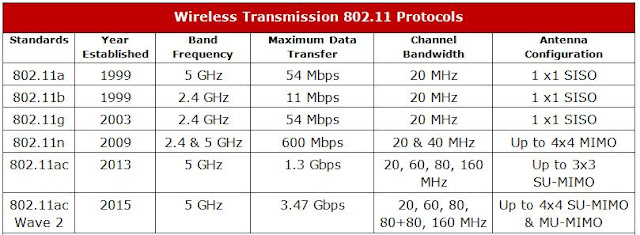
\includegraphics[width=0.8\textwidth]{figures/IEEE80211.png}
\end{figure}